\documentclass[../main.tex]{subfiles}

\begin{document}
\subsubsection{Active Learning Key Literature}
There exists a plethora of research within the AL area; however, due to the specific focus on medicine within this PhD, I will focus on existing literature within the medical domain and some key ones from others. It is valid to delineate between research within differing domains within AL (e.g., e-discovery in the Legal Domain, sentiment analysis on social media, or image classification in computer vision) as each domain presents unique challenges and characteristics that influence the application of AL techniques. In the medical domain, particularly in SRs, AL must contend with highly specialised vocabulary, complex interrelationships between concepts, and the critical importance of high recall to ensure that relevant studies are not missed.
The emphasis of the medical domain on evidence-based practice and the potential impact on patient care requires a more stringent approach to AL. Unlike other domains, where missing a small percentage of relevant items might be acceptable in systematic medicine reviews, overlooking a crucial study could have significant consequences. This requirement for near-perfect recall and the need to process large volumes of literature efficiently create a unique set of demands for medical TAR AL algorithms. This literature review will assess each work for their respective contributions, the datasets used, the evaluation metrics (and scores achieved), the models used, and the representation of data points used in each approach.

An early contribution to this field demonstrated that automated classification of document citations can be used to reduce the time reviewers spend screening evidence for inclusion in SRS of drug class efficacy \cite{cohen_reducing_2006}. The researchers used a novel data set created from annotated reference files from 15 SRs of drug classes. The features were extracted from the research articles using the "bag-of-words" approach for the title and abstract, the MeSH terms, and the MEDLINE publication type. The features were one-hot encoded and selected using the chi-square test to drop insignificant features. Finally, this input was used to train a perceptron model and was evaluated using precision, recall, and the F measure in a range of sample weighting and the WSS@95\%. This work's significant contribution was using machine learning approaches to address this screening issue.

A significant contribution to the field came from a simulation study that mimics the process of a human reviewer screening records while interacting with an active learning model \cite{ferdinands_performance_2023}. This work used six previously labelled SRs. It looked at four classification techniques (naive Bayes, logistic regression, support vector machines, and random forest). Two feature extraction strategies (TF-IDF and doc2vec) were evaluated based on the work saved on sampling and recall. The title and abstracts were used to generate these inputs. It showed that in a simulated approach, the models reduced the number of publications screened from 91.7 to 63. 9\% (WSS@95). The naive Bayes and TF-IDF models yielded the best overall results in this study. This study is limited due to the smaller datasets used and the feature extraction approaches used (which, for the year of publication, other potential superior choices, such as contextual embeddings, could have been explored). It introduced some new evaluation metrics, such as TTD and ATD. This research only superficially evaluates the variability of these approaches in SRs, reporting the range of WSS@95 and not attempting to consider factors within SRs that may have led to this variability. 

More recent work reported a protocol denoted ``CAL'' (Continuous Active Learning), initially performed on legal datasets \cite{cormack_evaluation_2014}. The process involves selecting an initial set of seed documents, typically using keyword search, which are then reviewed and coded. This training set is used to train a model that scores each document based on its response (relevant) likelihood. The top-scoring documents that have not been coded are then reviewed and coded. The extended training set is then used to retrain the model, and this process continues until ``enough'' of the responsive documents are found.
The key difference between this approach and previous ones, such as SAL (Simple Active Learning) and SPL (Simple Passive Learning), is their selection strategy: CAL uses relevance feedback (selecting highest-scoring documents), SAL uses uncertainty sampling, and SPL uses random selection. CAL achieved better results on the recall@75 % metric, which measures the effort required to achieve 75% recall.
The study primarily used SVM (Sofia-ML implementation of Pegasos SVM) for all protocols. It mentions briefly that it replicated most experiments using logistic regression, achieving similar results to SVM. It also tested with Nave Bayes, which achieved generally inferior results overall but maintained the same relative effectiveness among the protocols.
This paper is essential to outline the CAL process and demonstrate its effectiveness. However, it had some limitations: It used a fixed batch size of 1,000 documents for efficiency, though they noted slightly better results with a batch size of 100 for CAL. Although multiple classifiers were tested, detailed performance comparisons between models were not reported. The study did not explore extensively the effects of feature engineering methods. The human factors in review accuracy were not fully addressed in the simulation. Despite these limitations, the article provided a strong foundation for understanding and further investigating TAR protocols in SR TAR.

The follow-up was to introduce the autonomous TAR process (Auto TAR), which showed better performance than CAL \cite{cormack_autonomy_2015}. The algorithm is outlined in Figure \ref{fig:autotar_process}. 
The AUTO TAR process differs from CAL through:
\begin{itemize}
    \item AUTO TAR uses a single seed document, and CAL uses a 1,000 document set.
    \item AUTO TAR uses word-based features TF-IDF, and CAL uses binary byte-4 grammes.
    \item AUTO TAR exponentially increases batch sizes, starting with one and increasing by 10\% each iteration; CAL's batch size is fixed at 1,000
\end{itemize}

\begin{figure}
    \centering
    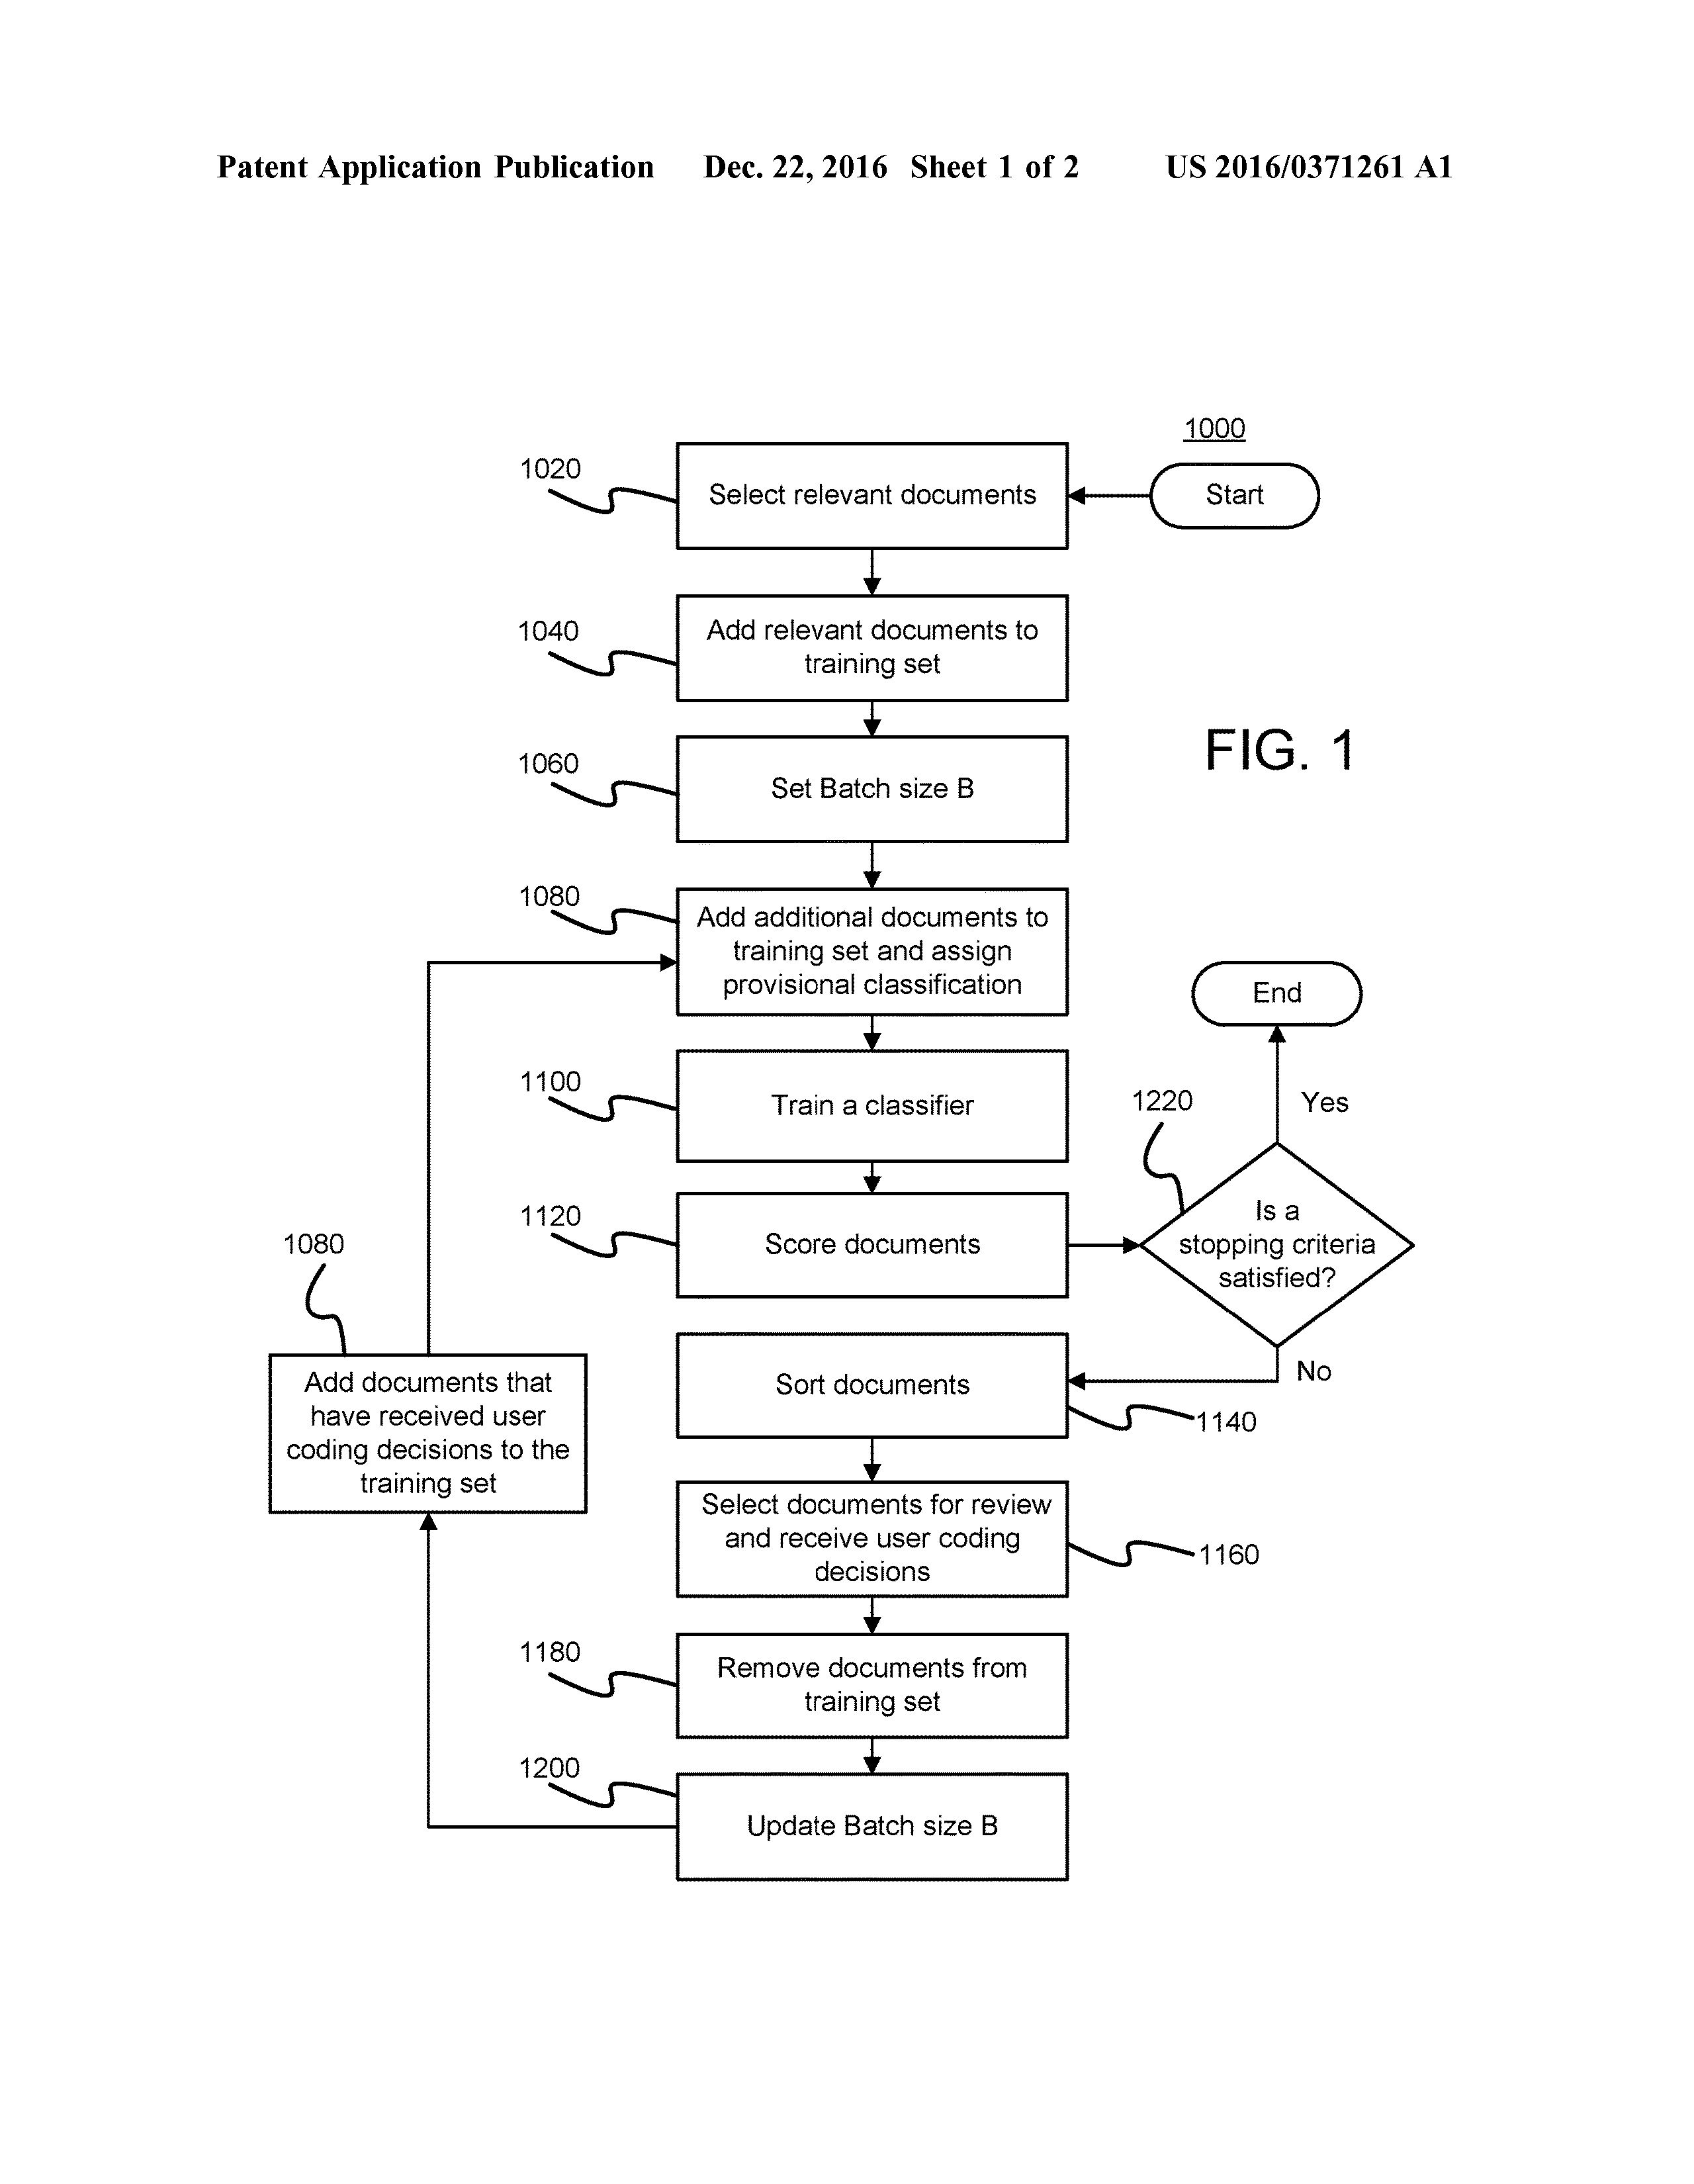
\includegraphics[width=1\linewidth]{sections//images/autotar.jpg}
    \caption{Auto TAR outline, as documented within the patient filing by Cormack et al. \cite{cormack_systems_2016}}.
    \label{fig:autotar_process}
\end{figure}
Finally, this approach was augmented to use BM25 (a saturated form of TF-IDF) + logistic regression and has been considered state-of-the-art for the past eight years. This is often referred to as "base model implementation", or abbreviated to BMI.

Since 2016's AutoTar approach, the transformer architecture has advanced virtually all fields within natural language processing, permeating almost every aspect of the field \cite{vaswani_attention_2023}. However, the TAR process has remained surprisingly resistant to these advances. Although a comprehensive analysis of transformer-based improvements is beyond the scope of this literature review, their primary advantage is their ability to provide a nuanced contextual understanding of written texts.
This contextual comprehension differs significantly from traditional feature extraction techniques such as TF-IDF. Transformers employ self-attention mechanisms to learn context-dependent text representations, enabling them to capture subtle semantic relationships and long-range dependencies not present with TF-IDF-like approaches, in the TAR process.

\hl{Add in about CALBERT}


Subsequent research using decoder architectures within CAL attempted to understand why their performance was underwhelming compared to BMI. 
Goldilocks \cite{yang_goldilocks_2022} took a pre-trained BERT model and fine-tuned it first on the unlabelled corpus (0-10 epochs were tested). They then randomly selected a positive example seed, and on each iteration of the AL process 200 documents were sampled using either relevance feedback or uncertainty sampling. During each iteration, after labelling, all labelled documents were used to fine-tune BERT again for 20 epochs, using the previous model from the previous iteration as the starting point. The input was the concatenated title and body text, truncated to 512 tokens. The model was then used to classify a document's relevance. They found that 5-epoch fine-tuning on the unlabelled dataset was "just right", and achieved similar performance to that of TF-IDF \& logistic regression within domain dataset (RCV1-V2 corpus), and statistically significantly worse on out-of-domain dataset(Jeb Bush corpus). Although not discussed in the paper, this could be explained through the phenomenon of "catastrophic forgetting", where too much fine-tuning on the task corpus might cause the model to forget useful general knowledge from pertaining \cite{xu_forget_2020}. Additionally, they used the model from the previous iteration as a starting point for new classification fine-tuning iterations, which could have further compounded this. 

However, the concept of a "goldilocks" epoch for CAL within medical data sets did not seem to hold, with subsequent research demonstrating that a "just right retaining epoch" was not present in the CLEF data set \cite{noauthor_ielabgoldilocks-reproduce_2024}. 

\hl{Issues with Goldilocks:}
\begin{enumerate}
    \item Contrived experimental design.
    \item Sensitive to pre-trained model choice.
\end{enumerate}


\end{document}